\documentclass[compress,11pt,xcolor=svgnames,aspectratio=169]{beamer}
\usetheme{Esiwace}
\usefonttheme[onlysmall]{structurebold}

%\usepackage{caption}
%\captionsetup{labelformat=empty, format=plain, labelsep=none,textfont=footnotesize}

\usepackage[utf8]{inputenc}
\usepackage[english]{babel}
\usepackage[T1]{fontenc}
\usepackage{eurosym}
%\usepackage{ulem}
\usepackage{listings}
\usepackage{ragged2e}
\usepackage{pgfgantt}
\usepackage{comment}
% \usepackage[backend=bibtex]{biblatex}
% \bibliography{io} % \footfullcite{jones00}
% \usepackage[numbers]{natbib}
\usepackage[absolute,overlay]{textpos}
\usepackage{varwidth}

\newcommand{\lr}[1]{\textcolor{cyan}{LR: #1}}
\setbeamercolor{bibliography item}{parent=palette primary}

\newcommand{\sectionIntro}{
\begin{frame}{Outline}
  \tableofcontents[currentsection,hideothersubsections]%,subsectionstyle=hide/hide/hide
\end{frame}
}

\newcommand{\sectionIntroHidden}{
\begin{frame}{Outline}
  \tableofcontents[currentsection,subsectionstyle=hide/hide/hide]
\end{frame}
}

\definecolor{gold}{rgb}{0.83, 0.69, 0.22}

\makeatletter
\renewcommand{\itemize}[1][]{%
  \beamer@ifempty{#1}{}{\def\beamer@defaultospec{#1}}%
  \ifnum \@itemdepth >2\relax\@toodeep\else
    \advance\@itemdepth\@ne
    \beamer@computepref\@itemdepth% sets \beameritemnestingprefix
    \usebeamerfont{itemize/enumerate \beameritemnestingprefix body}%
    \usebeamercolor[fg]{itemize/enumerate \beameritemnestingprefix body}%
    \usebeamertemplate{itemize/enumerate \beameritemnestingprefix body begin}%
    \list
      {\usebeamertemplate{itemize \beameritemnestingprefix item}}
      {\def\makelabel##1{%
          {%
            \hss\llap{{%
                \usebeamerfont*{itemize \beameritemnestingprefix item}%
                \usebeamercolor[fg]{itemize \beameritemnestingprefix item}##1}}%
          }%
        }%
      }
  \fi%
  \beamer@cramped%
  \justifying% NEW
  %\raggedright% ORIGINAL
  \beamer@firstlineitemizeunskip%
}
\makeatother

\tcbuselibrary{raster}

\DeclareGraphicsExtensions{.pdf,.png,.jpg,.jpeg}
\graphicspath{{./fig/}}

\title[Input/Output and Middleware -- Talk Session]{2020 Summer School on Effective HPC for Climate and Weather \\[0.5cm] Input/Output and Middleware}
\author[Pedro, Kunkel]{Luciana Pedro, Julian Kunkel
}
\institute[WP4 Team]{Department of Computer Science, University of Reading}
\date{18 June 2020}

\begin{document}

%%%%%%%%%%%%%%%%%%%%%%%%%%%%%%%%%%%%%%%%%%%%%%%%%%%%%%%%%%%%
\begin{frame}[plain]
    \titlepage
\end{frame}

%%%%%%%%%%%%%%%%%%%%%%%%%%%%%%%%%%%%%%%%%%%%%%%%%%%%%%%%%%%%
\begin{withoutheadline}
\begin{frame}{Outline}
    \begin{centering}
    \tableofcontents[hideallsubsections]
    \end{centering}

    \disclaimer
\end{frame}
\end{withoutheadline}

% Input/Output and Middleware
% Climate and weather research is typically data-intensive and applications must utilise input/output efficiently. Often, a user struggles to assess observed performance leading to superflux attempts to tune the application and optimise performance in a wrong layer of the stack. The content of this session is twofold. Firstly, we discuss storage layers focusing on the NetCDF middleware and provide a performance model that aids users to identify inefficient I/O. Secondly, we introduce the NetCDF Climate and Forecast (CF) conventions that are often used as a standard to exchange data.

\begin{frame}[fragile] {Learning Objectives}

\begin{itemize}
\setlength\itemsep{0.4cm}
  \item Discuss challenges for data-driven research (Section Introduction)
  \item Describe the role of middleware and file formats (Section Middleware)
  \item Identify typical I/O performance issues and their causes (Section I/O Performance)
  \item Apply performance models to assess and optimize the application I/O performance (Section I/O Performance)
  \item Design a data model for NetCDF/CF (Section NetCDF)
  \item Describe ongoing research activities in high-performance storage (Section Research Activities)
\end{itemize}

\end{frame}

\section{Introduction}
\sectionIntro

\subsection{I/O Bottleneck}

\begin{frame}[fragile] {I/O Bottleneck -- Example}

\begin{center}
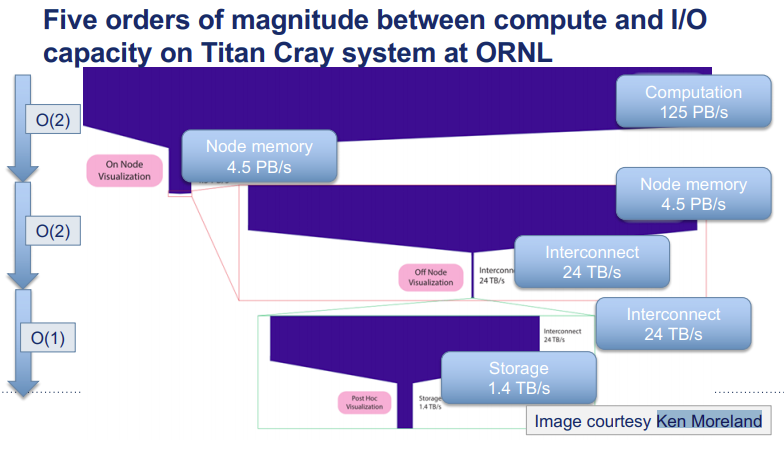
\includegraphics[scale=0.5]{fig/bottleneck-titan}
\end{center}

\lr{tut153s3}

\end{frame}

\begin{frame}[fragile] {I/O Bottleneck -- Historical Data}

\begin{itemize}

\item Kunkel et al. \cite{ESSAASOEKK14} analyze historical data from the German Climate Computing Center (DKRZ) and predict processor performance growth by 20x each generation ($\sim$5 years), while storage throughput/capacity improves by just 6x.

\end{itemize}

\begin{center}
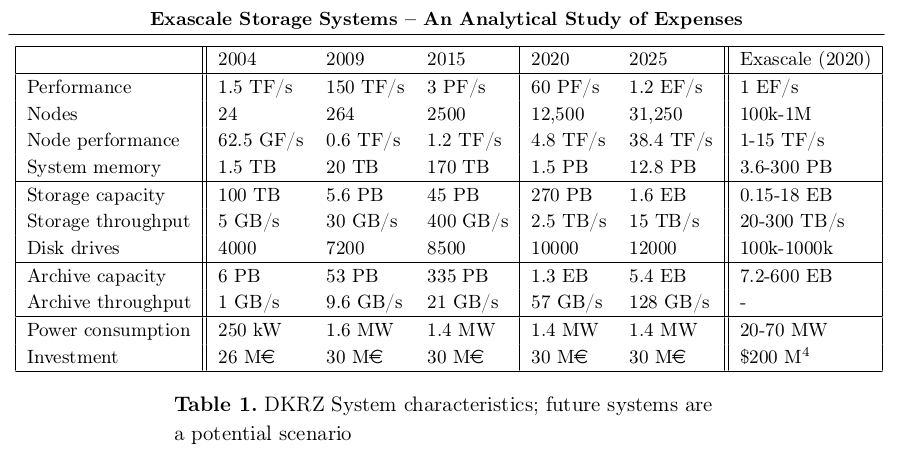
\includegraphics[scale=0.4]{fig/bottleneck-dkrz}
\end{center}

\nocite{ESSAASOEKK14}

\end{frame}

\begin{frame}[fragile] {Folders vs Metadata}

\begin{center}
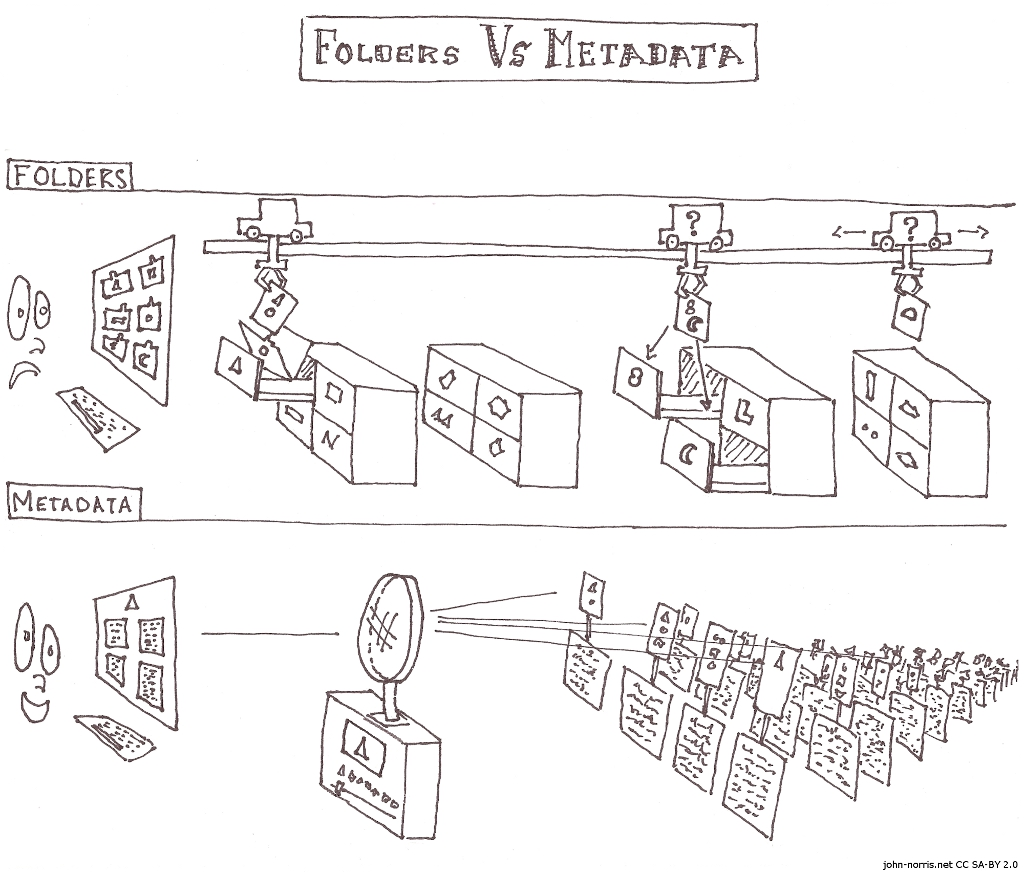
\includegraphics[scale=0.6]{fig/FoldersVsMeta}
\end{center}

\end{frame}

\subsection{Data-driven Research}

\begin{frame}[fragile] {Data-driven Research}

\begin{itemize}
\setlength\itemsep{0.4cm}

  \item \textbf{Data-driven Research} is the science of letting data tell us what we are looking for.
    \begin{itemize}
      \item \textbf{Database Management} is the science of efficiently storing and retrieving data.
      \item \textbf{Data Mining} is the science of discovering hidden correlations in data.
    \end{itemize}

  \item In HPC, the concerns of \textbf{storage} and \textbf{computing} are traditionally separated and optimised independently from each other and the needs of the end-to-end user.

  \item Workflows composed of data, computing, and communication-intensive tasks should drive interfaces and hardware configurations to best support the programming models.

  \item Data-driven workflows may benefit from the explicit and simultaneous use of a locally heterogeneous set of computing and storage technologies.

%  \item Many processes still require experts. For example, porting a workflow from one system to another still requires adjusting runtime parameters of applications and deciding on how data is managed.

\end{itemize}

\nocite{01403233}

\nocite{JSFI309}

\end{frame}

\section{Input/Output}
\sectionIntro

\subsection{Input/Output}

\begin{frame}[fragile] {Input/Output}

\begin{itemize}
\setlength\itemsep{0.3cm}

    \item Input/Output (I/O) is simply data migration.

    \begin{itemize}
      \item Memory $\Leftrightarrow$ Disk
    \end{itemize}

    \item I/O is a very expensive operation!

%    \begin{itemize}
%      \item Interactions with data in memory and on disk.
%    \end{itemize}

    \item How is I/O performed?

    \begin{itemize}

      \item I/O Pattern

      \begin{itemize}
        \item Number of processes and files.
        \item Characteristics of file access.
      \end{itemize}

    \end{itemize}

    \item Where is I/O performed?

    \begin{itemize}
      \item Characteristics of the computational system.
      \item Characteristics of the file system.
    \end{itemize}

\end{itemize}

\nocite{PIOTAPO12}

\end{frame}

\begin{frame}[fragile] {I/O Performance}

\begin{itemize}
\setlength\itemsep{0.5cm}

  \item There is no ``One Size Fits All'' solution to the I/O problem.

  \item Bottlenecks in performance can occur in many locations.

  \begin{itemize}
    \item Application and/or file system.
  \end{itemize}

  \item Many I/O patterns work well for some range of parameters.

  \item Going to extremes with an I/O pattern will typically lead to problems.

  \item {\color{gold}\textbf{Golden Rule:}} \lr{Increase performance by decreasing the number of I/O operations (latency) and increasing size (bandwidth).}

\end{itemize}

\nocite{PIOTAPO12}

\end{frame}

\begin{frame}[fragile] {I/O Types}

\begin{center}
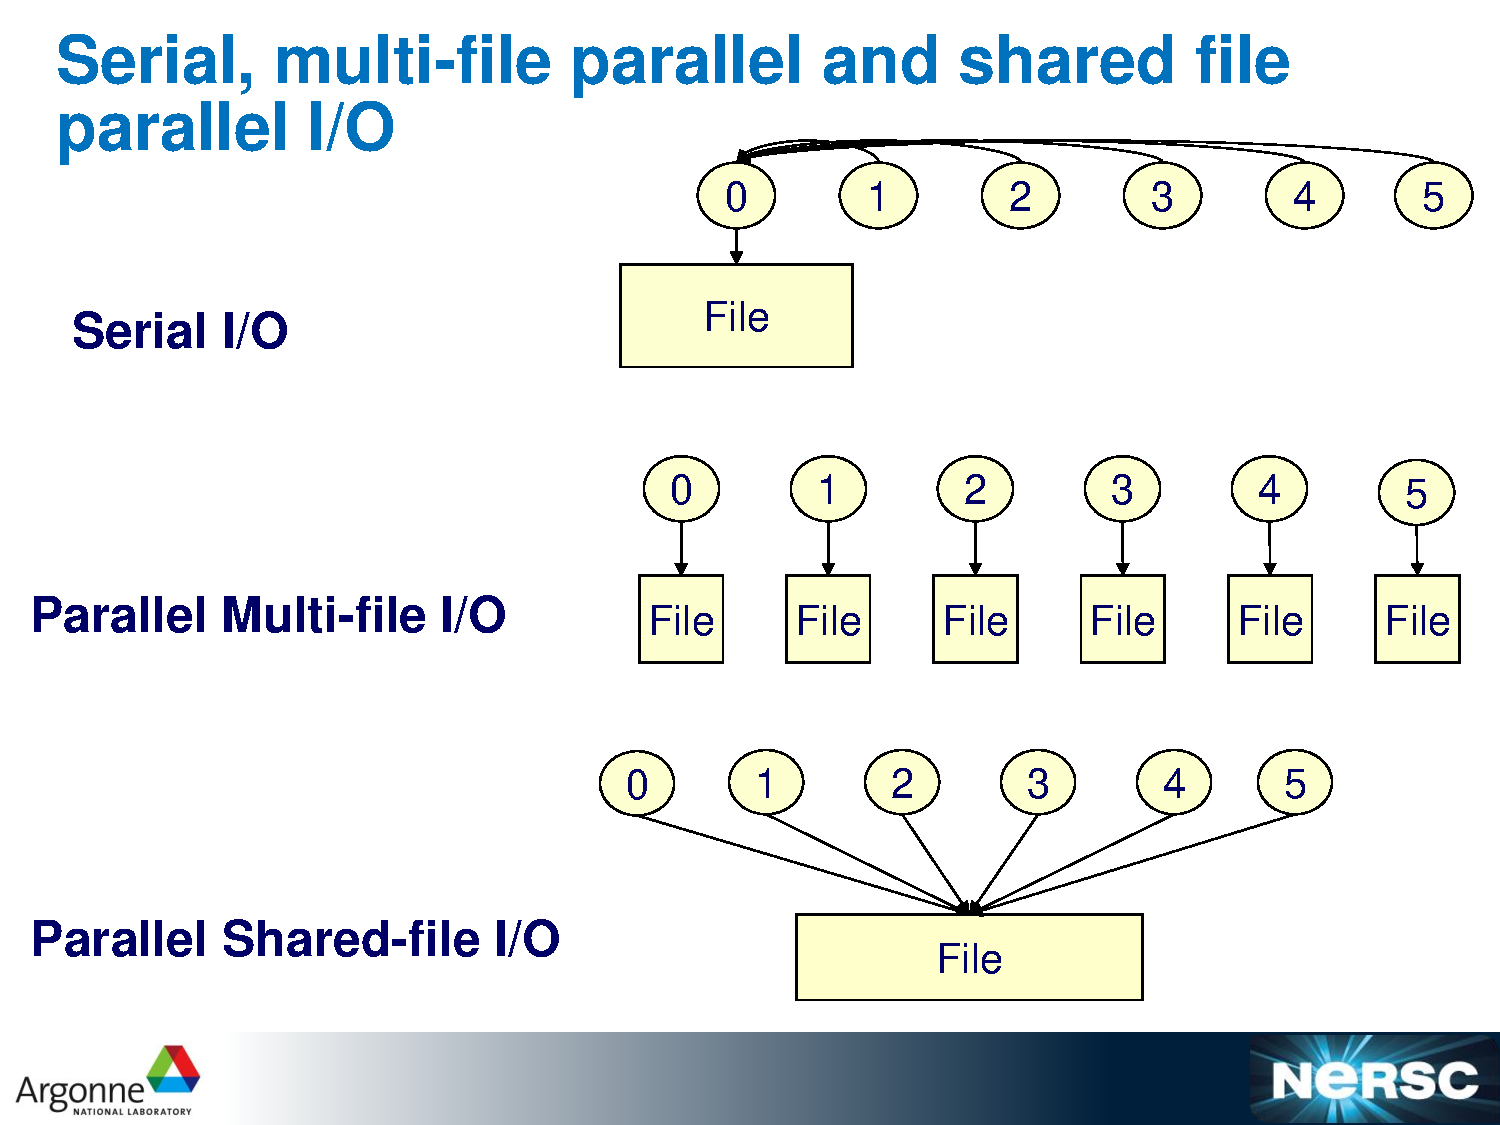
\includegraphics[scale=0.3]{io-types}
\end{center}

\lr{tut145s3}

\end{frame}

\begin{frame}[fragile] {I/O Access Patterns \lr{(Double-check the last two)}}

\begin{center}
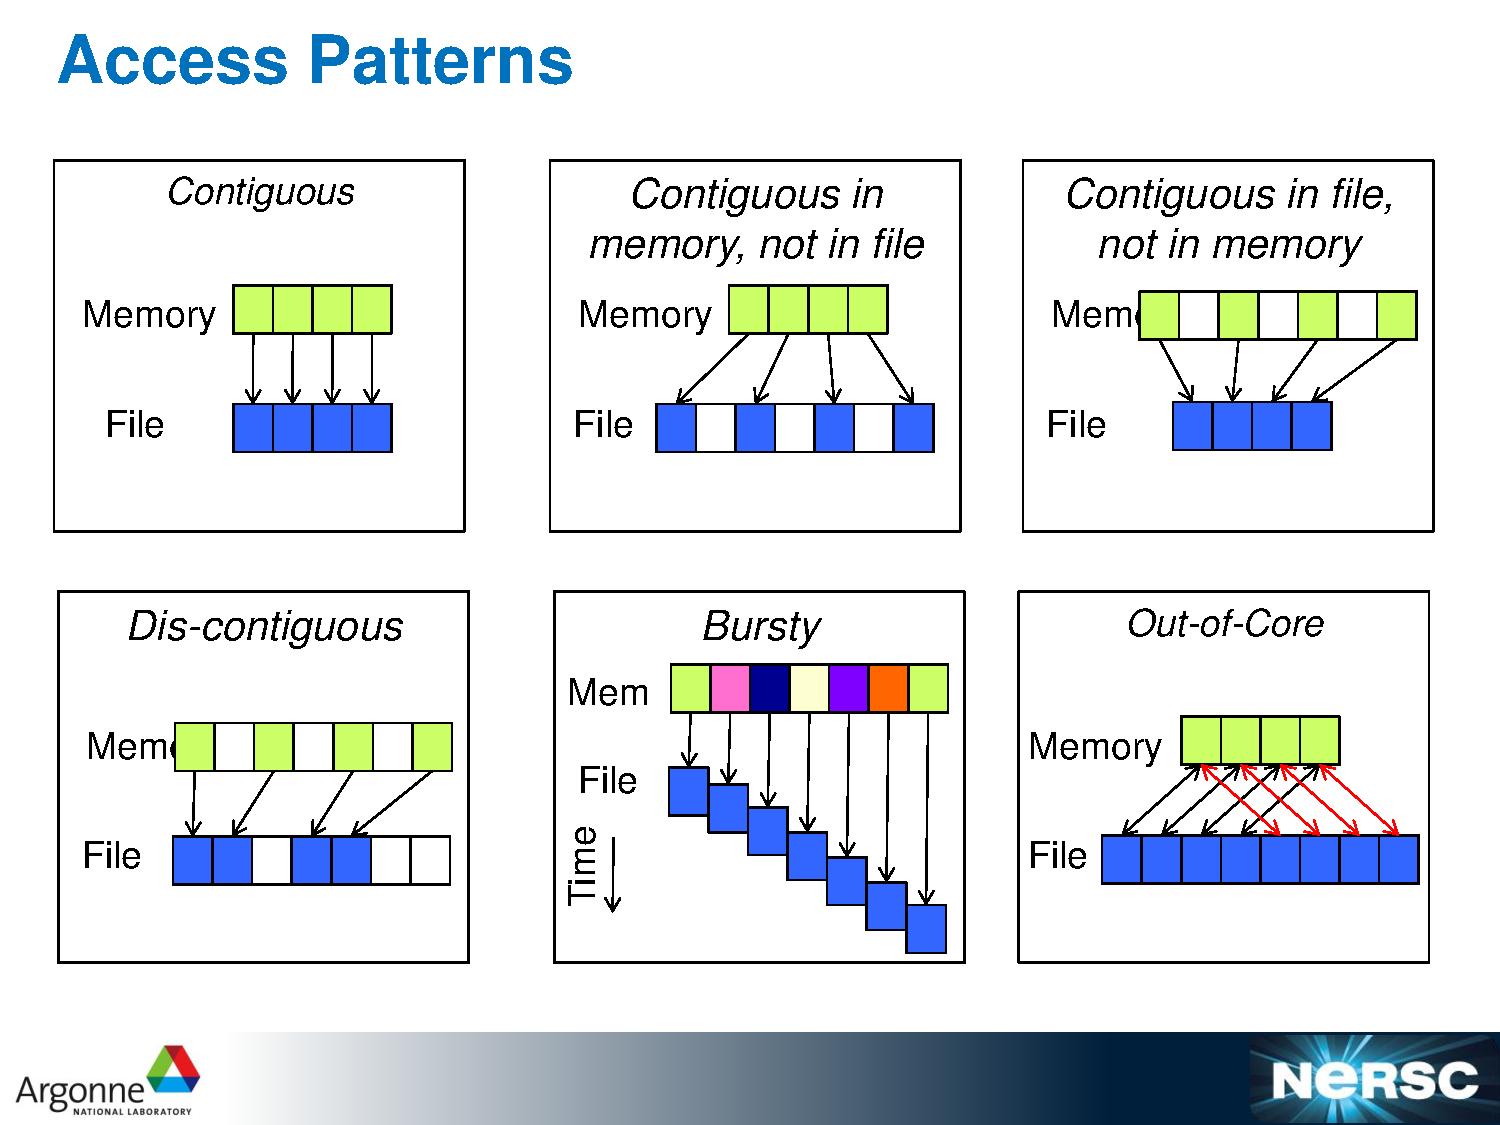
\includegraphics[scale=0.3]{io-patterns}
\end{center}

\lr{tut145s3}

\end{frame}

\begin{frame}[fragile] {File Striping}

\begin{center}
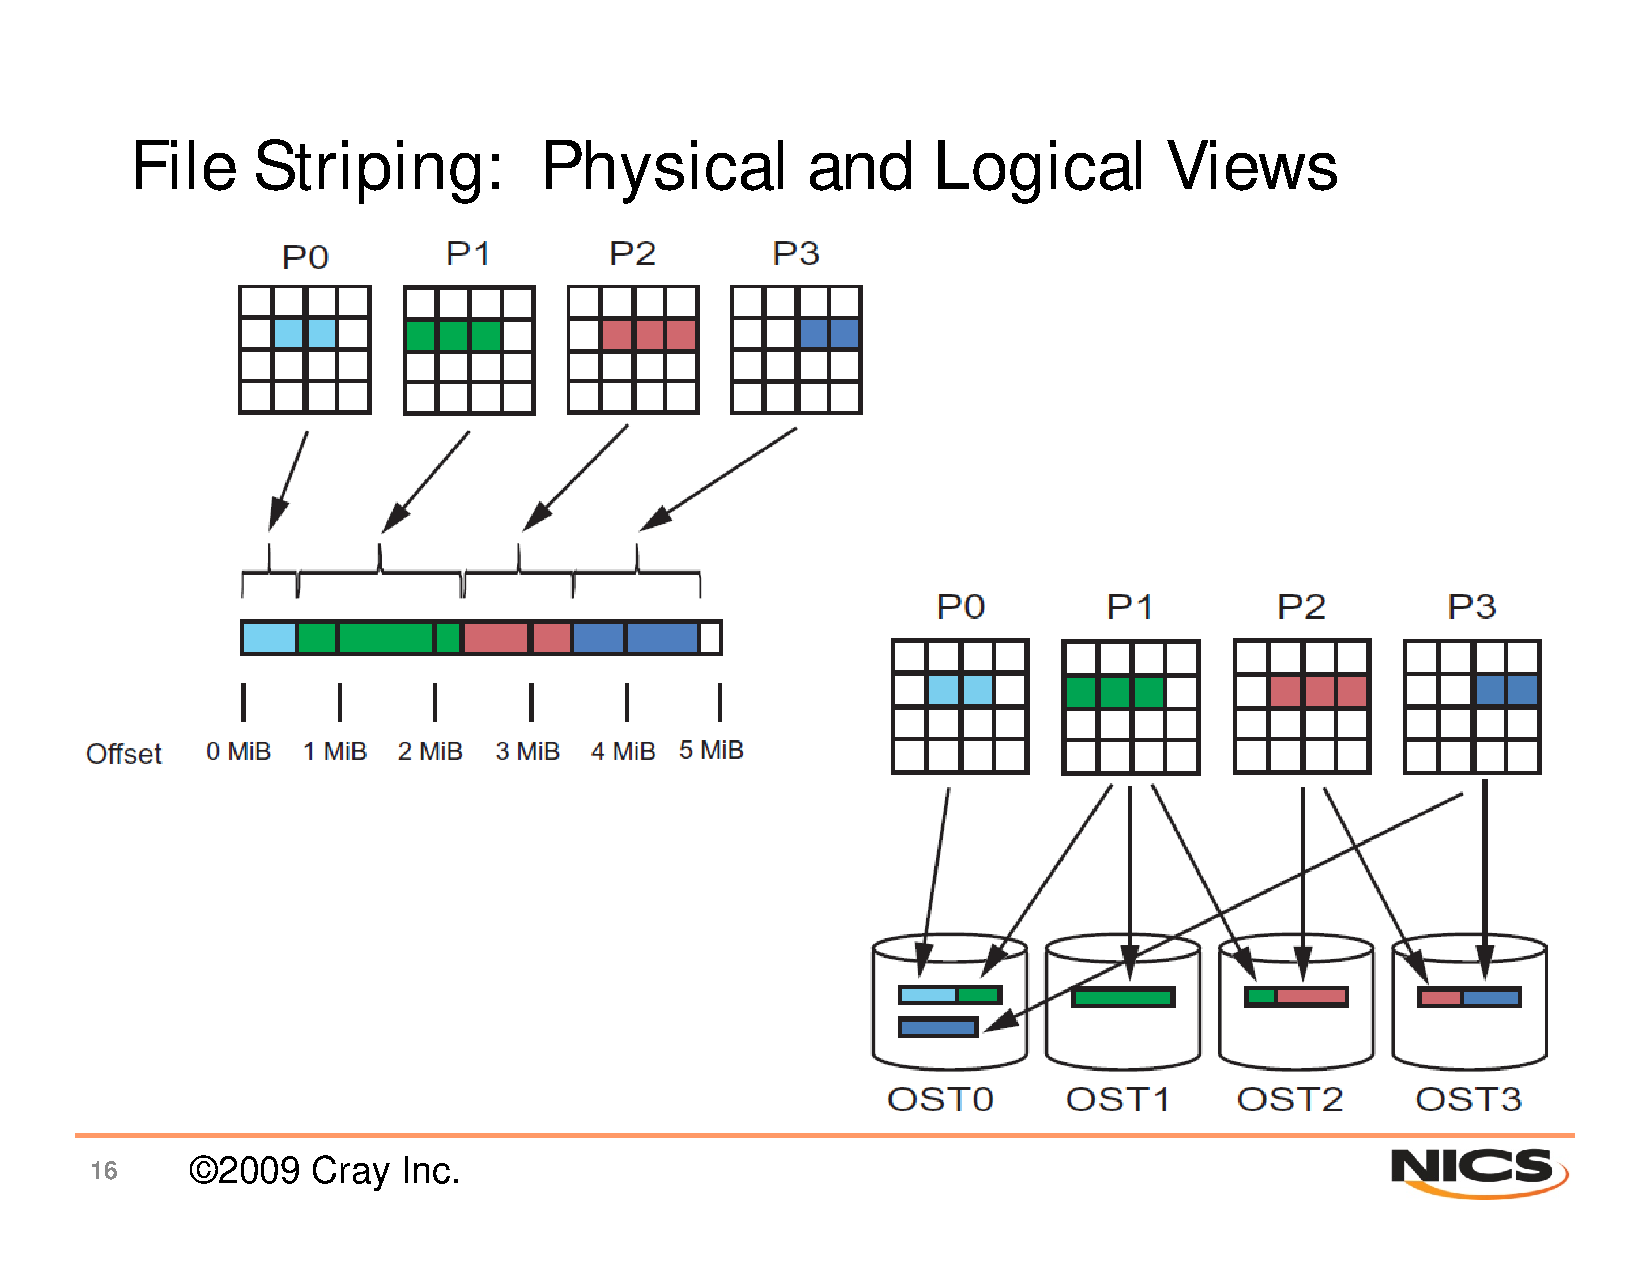
\includegraphics[scale=0.3]{file-striping}
\end{center}

\nocite{PIOTAPO12}

\end{frame}

\begin{frame}[fragile] {I/O Problems}

\begin{itemize}
\setlength\itemsep{0.7cm}

\item Not enough I/O capacity on current HPC systems, and the trend is getting worse.

\item If there is not enough I/O, you can not write data% to storage
, so you can not analyze it.
    \begin{itemize}
        \item Lost science!
    \end{itemize}

\item Energy consumption: it costs a lot of power to write data to disk.

\item Opportunity for doing better science (analysis) when have access to full spatiotemporal resolution data.\lr{What does that mean?}

\end{itemize}

\begin{center}
%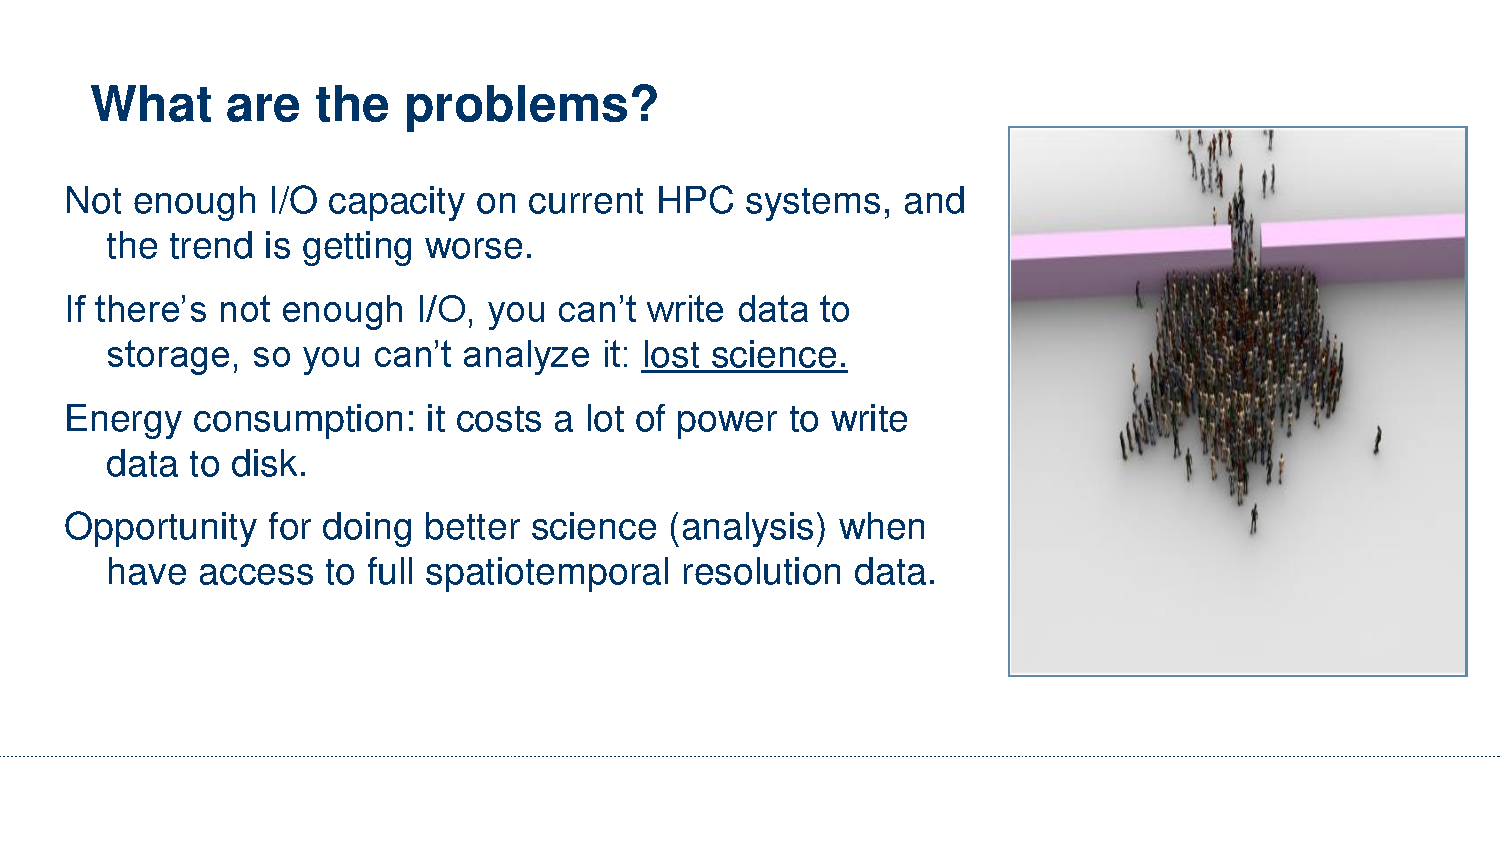
\includegraphics[scale=0.5]{io-probs}
\end{center}

\lr{tut153s3}

\end{frame}

\begin{frame}[fragile] {Challenges in Application I/O \lr{(== I/O Applications)}}

\begin{itemize}
\setlength\itemsep{0.4cm}

\item \lr{Leverage aggregate communication and I/O bandwidth of clients}
    \begin{itemize}
        \item \lr{... but not overwhelming a resource limited I/O system with uncoordinated accesses!}
    \end{itemize}

\item Limit the number of files that must be managed.

\item Avoid unnecessary post-processing. \lr{(why?)}

\item Interact with storage through convenient abstractions.
    \begin{itemize}
      \item Store in portable formats!
    \end{itemize}

\item {\color{gold}\textbf{Golden Rule:}} Parallel I/O software is available and they can address all
of these problems, when used appropriately.

\end{itemize}

%\begin{center}
%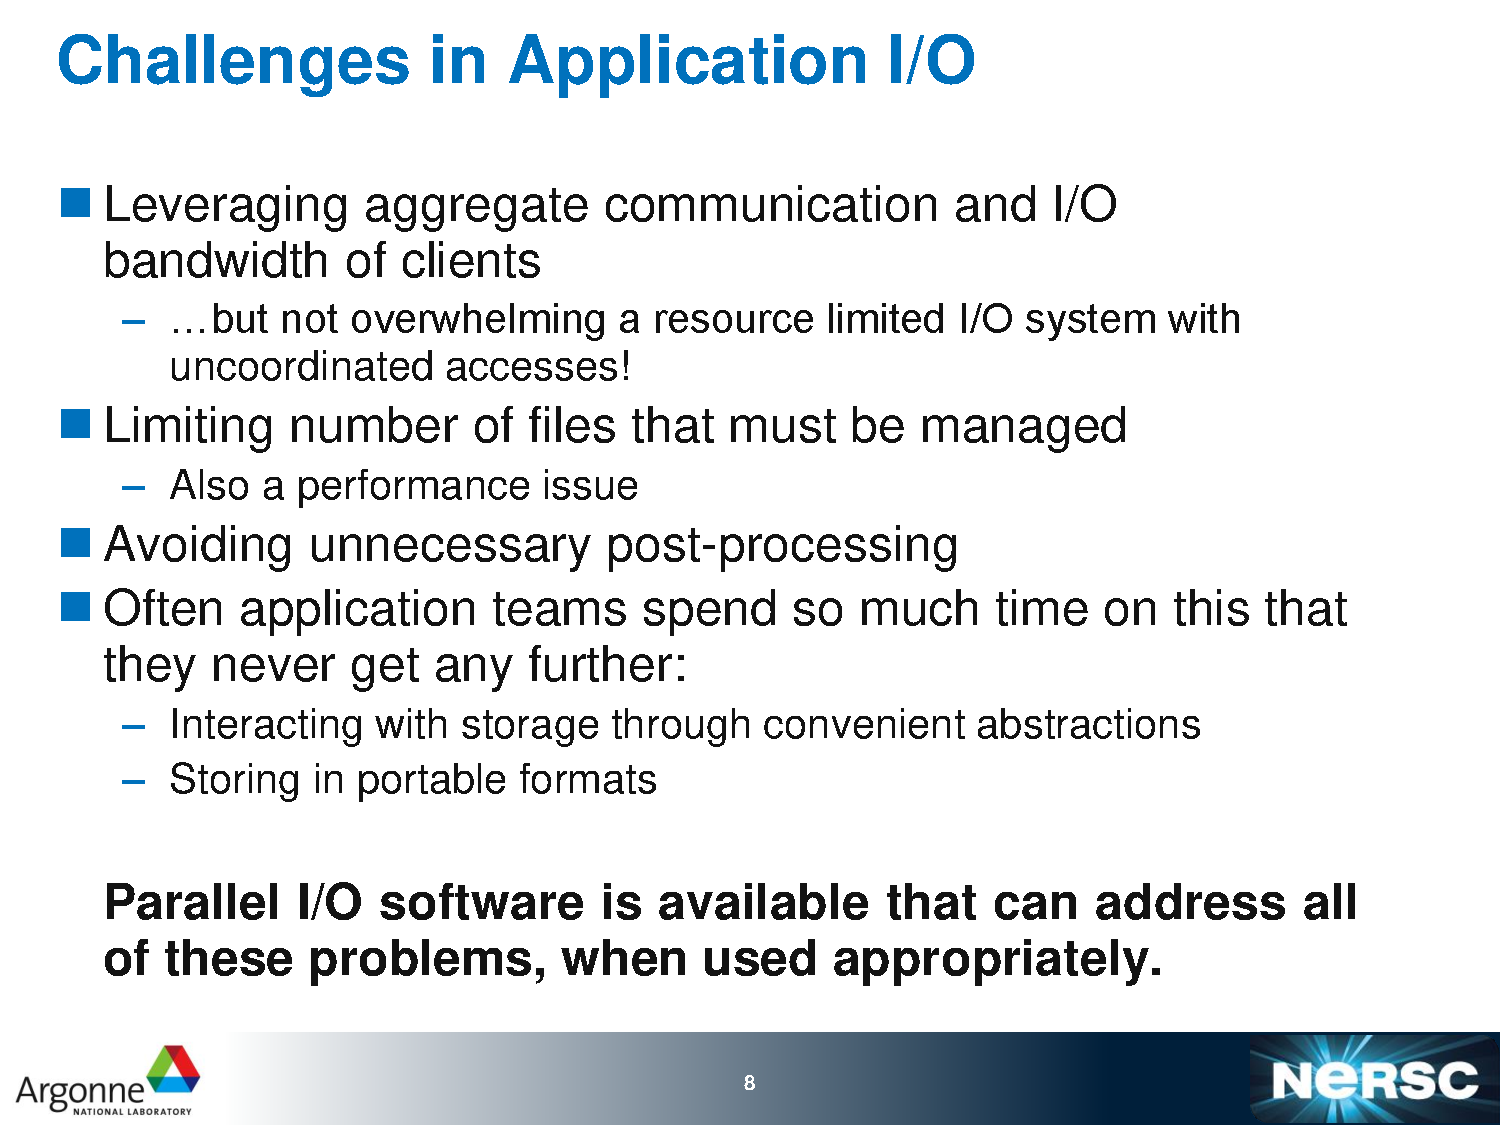
\includegraphics[scale=0.5]{fig/challenges-io}
%\end{center}

\lr{tut145s3}

\end{frame}

\section{Middleware}
\sectionIntro

\subsection{Introduction}

\begin{frame}[fragile] {Middleware}

\begin{itemize}
\setlength\itemsep{0.4cm}

  \item Middleware is software occupying a middle position between application programs and operating systems.\lr{What is this database table in the picture? Just a common database for the application?}

  \begin{center}
  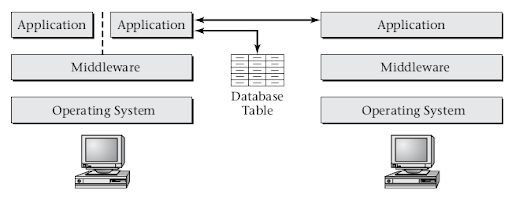
\includegraphics[scale=0.5]{fig/middleware}
  \end{center}

  \item Common middleware examples include relational database systems, application server middleware, message-oriented middleware, web middleware, and transaction-processing monitors.\lr{Famous "brand" examples? I couldn't find any...}

\end{itemize}

\lr{osm-rev1.3.1 1.3}

\end{frame}

\begin{frame}[fragile] {Middleware}

\begin{itemize}
\setlength\itemsep{0.6cm}

  \item Middleware is in the middle of the vertical stack, between the application programs and the operating system.

  \item Viewed horizontally rather than vertically, middleware is also in the middle of interactions between different application programs (possibly even running on different computer systems), because it provides mechanisms to support controlled interaction through coordination, persistent storage, naming, and communication.\lr{Link ESDM here!}

  \item Middleware provide a more sophisticated form of persistent storage than the standard supported by most operating systems.\lr{Is this true for all types of middleware?}

\end{itemize}

\lr{osm-rev1.3.1 1.3}

\end{frame}

\begin{frame}[fragile] {Describe the role of middleware and file formats}

\begin{itemize}

  \item File formats
    \begin{itemize}
        \item
        \item
    \end{itemize}

  \item
    \begin{itemize}
      \item
    \end{itemize}

\end{itemize}

\end{frame}

\subsection{I/O Solutions}

\begin{frame}[fragile] {I/O Solutions}

\begin{itemize}

\item As we are moving towards exascale, the gap between computing power and I/O bandwidth will
widen and researchers are looking for solutions to tackle this problem.\\[0.4cm]

\item There are essentially three lines of research:\\[0.4cm]

    \begin{itemize}
    \setlength\itemsep{0.6cm}

      \item at hardware level,
      \item at middleware level,\lr{Link ESDM here!}
      \item and at application level.

    \end{itemize}

\end{itemize}

\nocite{3372390}

\end{frame}

\begin{frame}[fragile] {Hardware Level}

\begin{itemize}

    \item Non-volatile memory (NVM)\\[0.4cm]

    \begin{itemize}
    \setlength\itemsep{0.6cm}

        \item Non-volatile memory (NVM) is a type of computer memory that can retrieve stored information even after having been power cycled.

        \item The capabilities of NVM (i.e., capacity, bandwidth, energy consumption) are somewhere in-between main memory and persistent storage, thus it is often used as a ``caching'' solution between these two layers.

        \item Examples of non-volatile memory include flash memory, read-only memory (ROM), ferroelectric RAM, most types of magnetic computer storage devices (e.g. hard disk drives, floppy disks, and magnetic tape), optical discs, and early computer storage methods such as paper tape and punched cards.

    \end{itemize}

\end{itemize}

\nocite{3372390}

\end{frame}

\begin{frame}[fragile] {Hardware Pop Quiz -- Non-volatile Memory}

\begin{center}

\begin{tabular}{cc}

\begin{tabular}{ccc}
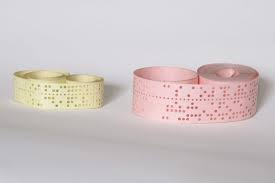
\includegraphics[scale=0.2 ]{fig/paper-tape} &
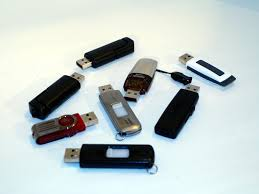
\includegraphics[scale=0.2 ]{fig/usb} &
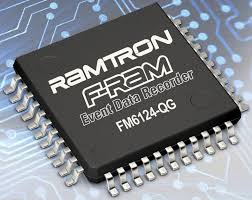
\includegraphics[scale=0.2 ]{fig/fram} \\
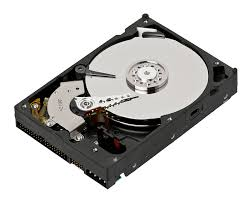
\includegraphics[scale=0.2 ]{fig/disk} &
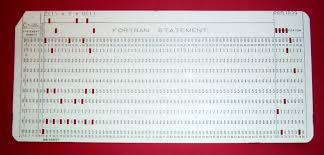
\includegraphics[scale=0.2 ]{fig/punch-card} &
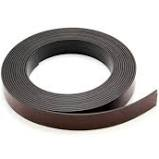
\includegraphics[scale=0.2 ]{fig/tape} \\
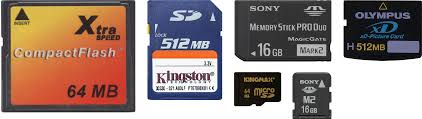
\includegraphics[scale=0.2 ]{fig/card} &
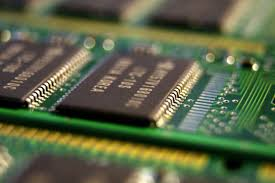
\includegraphics[scale=0.2 ]{fig/rom} &
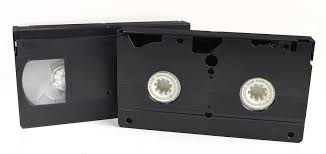
\includegraphics[scale=0.2 ]{fig/vhs} \\
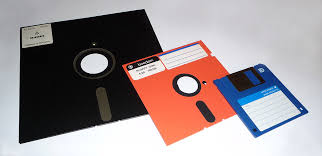
\includegraphics[scale=0.2 ]{fig/floppy} &
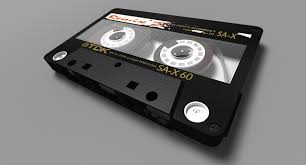
\includegraphics[scale=0.2 ]{fig/k7} &
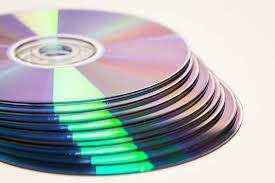
\includegraphics[scale=0.2 ]{fig/cd} \\
\end{tabular}

\end{tabular}

\end{center}

\end{frame}

\begin{frame}[fragile] {Hardware Pop Quiz -- Non-volatile Memory}

\begin{center}

\begin{tabular}{cc}

\begin{tabular}{ll}
A & \parbox{4cm}{flash memory}\\
B & read-only memory\\
C & ferroelectric RAM\\
D & hard disk drives\\
E & floppy disks\\
F & magnetic tape\\
G & optical discs\\
H & paper tape\\
I & punched cards\\
\end{tabular}

&

\begin{tabular}{ccc}
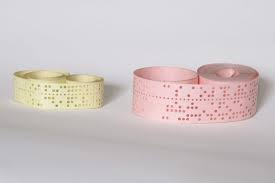
\includegraphics[scale=0.15]{fig/paper-tape} &
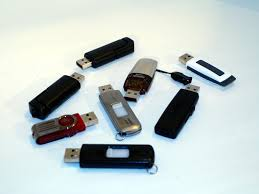
\includegraphics[scale=0.15]{fig/usb} &
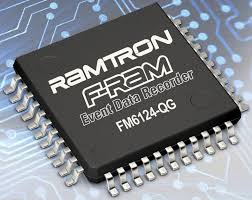
\includegraphics[scale=0.15]{fig/fram} \\
1 & 2 & 3 \\
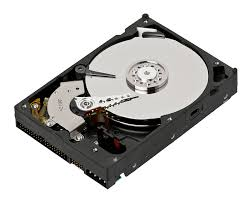
\includegraphics[scale=0.15]{fig/disk} &
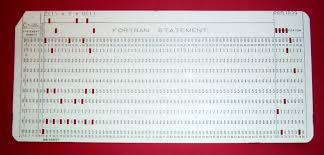
\includegraphics[scale=0.15]{fig/punch-card} &
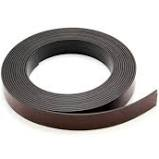
\includegraphics[scale=0.15]{fig/tape} \\
4 & 5 & 6 \\
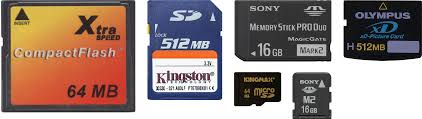
\includegraphics[scale=0.15]{fig/card} &
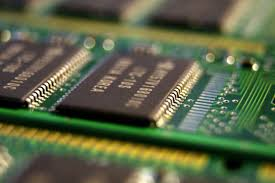
\includegraphics[scale=0.15]{fig/rom} &
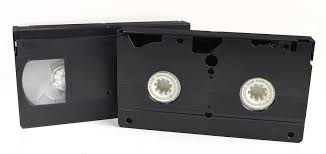
\includegraphics[scale=0.15]{fig/vhs} \\
7 & 8 & 9 \\
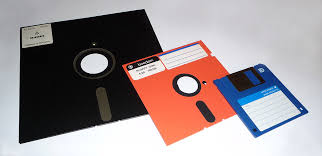
\includegraphics[scale=0.15]{fig/floppy} &
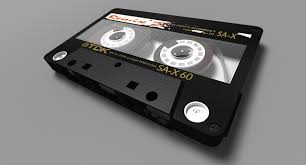
\includegraphics[scale=0.15]{fig/k7} &
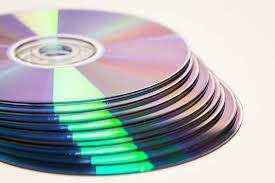
\includegraphics[scale=0.15]{fig/cd} \\
10 & 11 & 12 \\
\end{tabular}

\end{tabular}

\end{center}

\end{frame}

\begin{frame}[fragile] {Hardware Pop Quiz -- Non-volatile Memory}

\begin{center}

\begin{tabular}{cc}

\begin{tabular}{ll}
A & \parbox{4cm}{flash memory -- 2/7}\\
B & read-only memory -- 8\\
C & ferroelectric RAM -- 3\\
D & hard disk drives -- 4\\
E & floppy disks -- 10\\
F & magnetic tape -- 6/9/11\\
G & optical discs -- 12\\
H & paper tape -- 1\\
I & punched cards -- 5\\
\end{tabular}

&

\begin{tabular}{ccc}
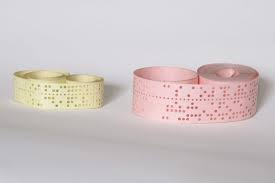
\includegraphics[scale=0.15]{fig/paper-tape} &
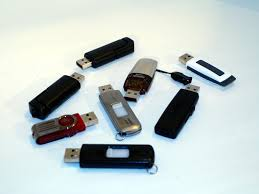
\includegraphics[scale=0.15]{fig/usb} &
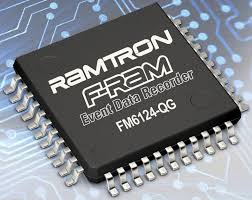
\includegraphics[scale=0.15]{fig/fram} \\
1 & 2 & 3 \\
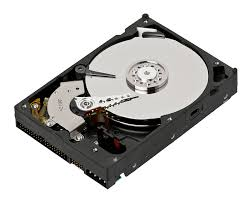
\includegraphics[scale=0.15]{fig/disk} &
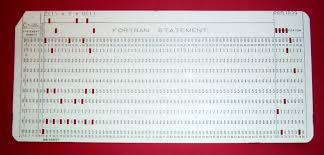
\includegraphics[scale=0.15]{fig/punch-card} &
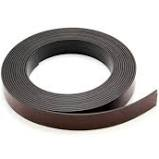
\includegraphics[scale=0.15]{fig/tape} \\
4 & 5 & 6 \\
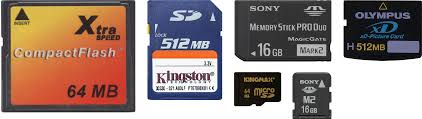
\includegraphics[scale=0.15]{fig/card} &
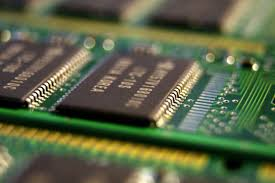
\includegraphics[scale=0.15]{fig/rom} &
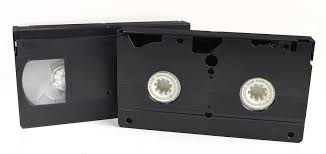
\includegraphics[scale=0.15]{fig/vhs} \\
7 & 8 & 9 \\
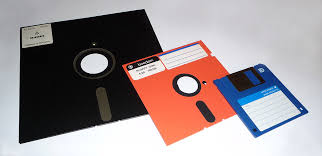
\includegraphics[scale=0.15]{fig/floppy} &
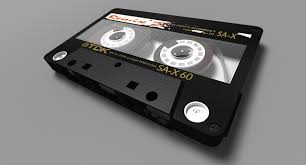
\includegraphics[scale=0.15]{fig/k7} &
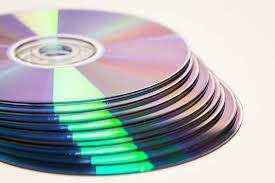
\includegraphics[scale=0.15]{fig/cd} \\
10 & 11 & 12 \\
\end{tabular}

\end{tabular}

\end{center}

\end{frame}

\begin{frame}[fragile] {Hardware Level}

\begin{itemize}

    \item Burst buffer (BB)\\[0.4cm]

      \begin{itemize}
      \setlength\itemsep{0.3cm}

      \item Burst buffer (BB) is a fast and intermediate storage layer positioned between the front-end computing processes and the back-end storage systems.

      \item HPC applications often show bursty I/O behavior (i.e., all processes read/write at the same time) and burst buffers help to absorb these workloads.

      \item Burst buffer is built from arrays of high-performance storage devices, such as NVRAM and SSD.

      \begin{center}
      \begin{tabular}{ccccc}
      \raisebox{1cm}{NVRAM} &
      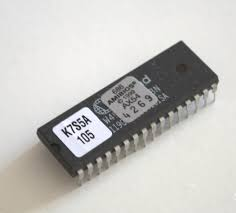
\includegraphics[scale=0.25]{fig/nvram} & $\qquad$ &
      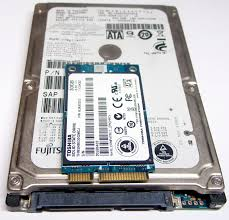
\includegraphics[scale=0.24]{fig/ssd} &
      \raisebox{1cm}{
        \begin{tabular}{c}
        SSD \\
        (on top of \\
        a hard drive)
        \end{tabular}
      }
      \end{tabular}
      \end{center}

      \end{itemize}

\end{itemize}

\nocite{3372390}

\end{frame}

\begin{frame}[fragile] {Hardware Level \lr{(Keep it?)}}

\begin{itemize}

      \item Multi-layer Storage Hierarchy (Examples)\\[0.4cm]

        \begin{itemize}
        \setlength\itemsep{0.6cm}

        \item Attached SSDs to compute nodes to aggregate many small I/O requests into few larger ones and/or to compute nodes to speed-up MPI-IO.

        \item Multi-layer storage hierarchy with NVM, SSDs, and different types of hard disks. % drives.

        \item Fast Forward Storage and IO (FFSIO), SAGE, Distributed Application Object Store (DAOS), Post-Petascale File System (PPFS), Scalable Object-Centric Metadata Management (SoMeta), Extensible Metadata Provider for Extreme-Scale Scientific Simulations (EMPRESS), Týr

        \item ECP [16], Fast-Forward [44], ADIOS [72], HDF VOL [29], ESiWACE [20], NEXTGenIO [69] and SAGE [78]

        \item Blue gene active storage, Dash

        \end{itemize}

\end{itemize}

\nocite{3372390}

\end{frame}

\begin{frame}[fragile] {Middleware Level}

\begin{itemize}
\setlength\itemsep{0.4cm}

\item Solutions in I/O middleware.

    \begin{itemize}

    \item E.g., file systems, I/O interfaces.\lr{Is a file systems an I/O middleware?}

    \end{itemize}

\item \textbf{Damaris:} Software framework that overlaps computation and I/O operations by dedicating a single core to I/O tasks.

\item \textbf{ADIOS:} I/O abstraction framework for HPC applications that enables switching between different I/O transport methods with little modification to application code and enabling integration of new I/O solutions.

\item \textbf{DeltaFS:} File systems that improves the scalability of file systems by letting compute nodes manage metadata instead of a centralized server.

\end{itemize}

\nocite{3372390}

\end{frame}

\begin{frame}[fragile] {Application Level}

\begin{itemize}

\item In-situ analysis\\[0.4cm]

    \begin{itemize}
    \setlength\itemsep{0.6cm}

    \item In biology and biomedical engineering, in situ means to examine the phenomenon exactly in place where it occurs (i.e., without moving it to some special medium).

    \item Rather than applications writing their raw output to storage to later be read again for post-processing (e.g., visualization, filtering, statistics), in-situ processing removes this overhead by performing the analysis directly on the same machines as where the applications run.

    \item ParaView, Dax, and Damaris/Viz are tools for large-scale in-situ visualization.\lr{Use that style in middleware?}

    \end{itemize}

\end{itemize}

\nocite{3372390}

\end{frame}

\begin{frame}[fragile] {Discussion\lr{Keep just this slide?}}

\begin{itemize}
\setlength\itemsep{0.2cm}

\item No one-size-fits-all solution to the storage problem and programmers must take I/O into careful consideration when developing applications.

\item Mismatch between the massive computational performance of processors and relatively limited I/O bandwidth of storage systems.

\item Three methods to alleviate this problem: new hardware technology, new I/O middleware, and application-specific solutions.

\item Hardware technology shows promising solutions, but different systems might employ different solutions, reducing the portability and increasing the complexity. % of software.

\item Middleware can alleviate some of this complexity with solutions such as ADIOS.

\item In-situ analysis is an example of how application-specific solutions can be used to improve I/O throughput and thus application performance.

\end{itemize}

\nocite{3372390}

\end{frame}

\section{I/O Performance}
\sectionIntro

\subsection{Introduction}

\begin{frame}[fragile] {I/O Performance}

\begin{itemize}
\setlength\itemsep{0.8cm}

  \item There are several aspects involved in delivering high I/O performance to parallel applications, from hardware characteristics to methods that manipulate workloads to improve achievable performance.

  \item Running the same application with different I/O configurations gives the possibility to tune the I/O system according to the application access pattern.

  \item One way to predict application performance in HPC systems with different I/O configurations is by using modeling and simulation techniques.

\end{itemize}

\nocite{SOPPOAASLK13}

\end{frame}

\begin{frame}[fragile] {I/O Stack}

\begin{center}
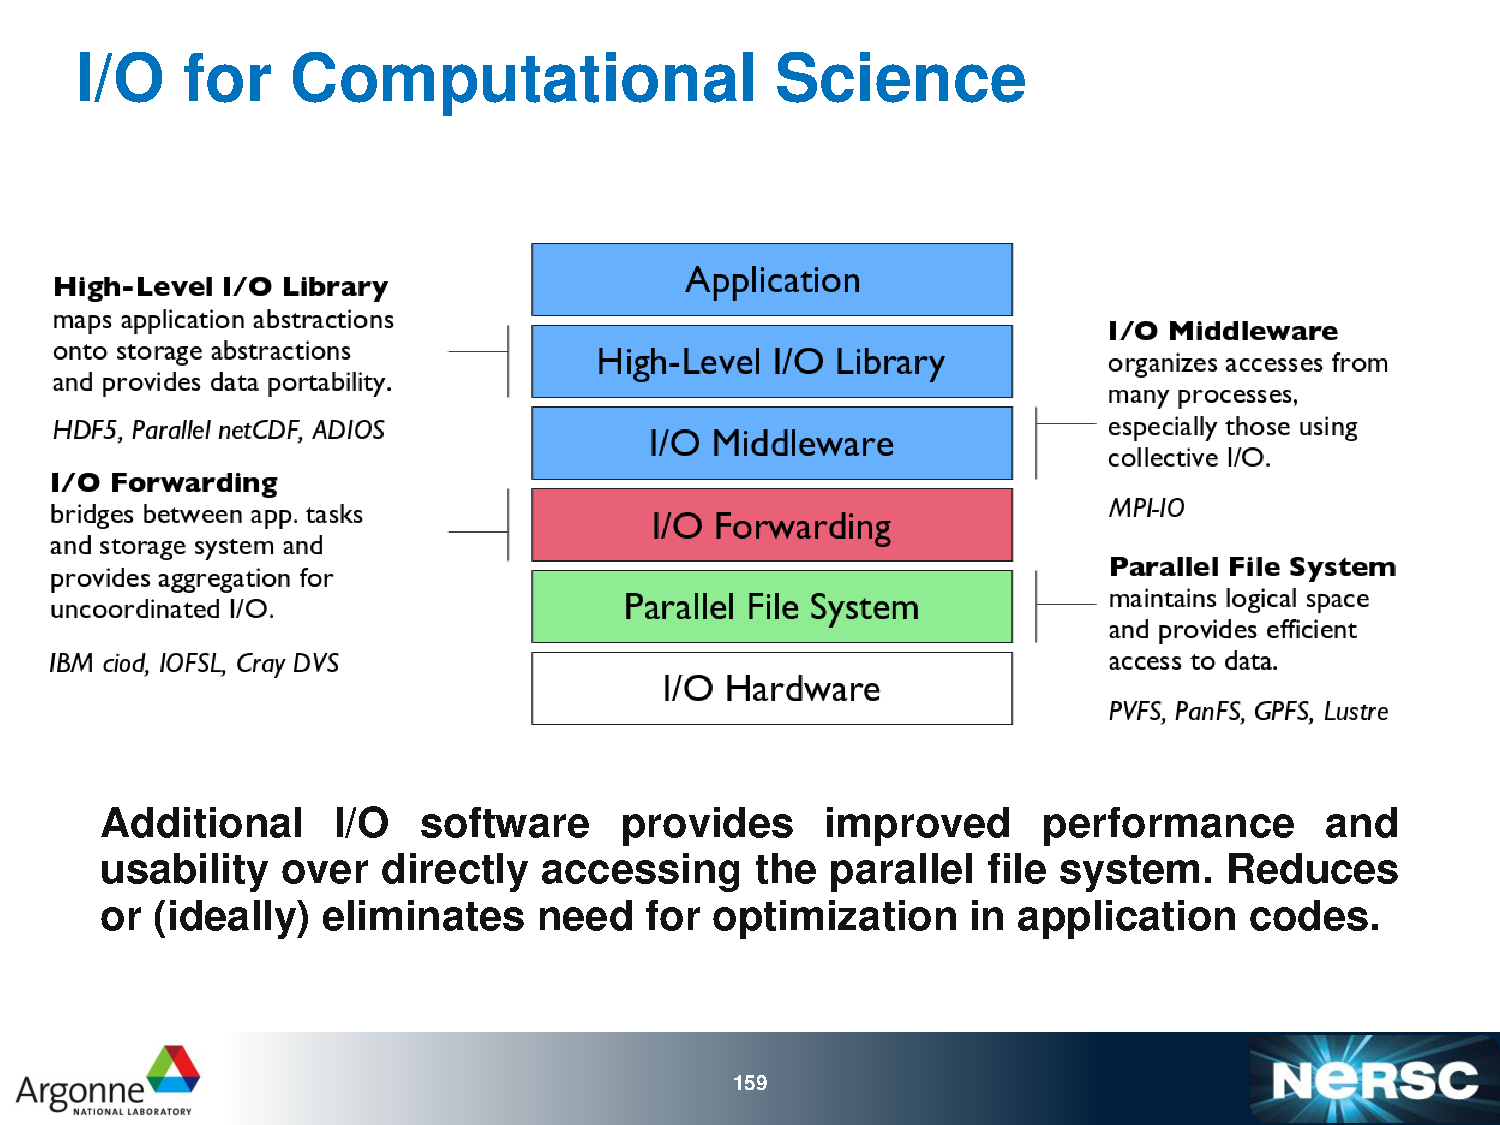
\includegraphics[scale=0.4]{fig/io-stack2}
\end{center}

\lr{Insert explanation about each leavel? Keep only the picture.}

\lr{tut145s3}

\end{frame}

\subsection{Typical Performance Factors}

\begin{frame}[fragile] {Typical Performance Factors}

\begin{center}
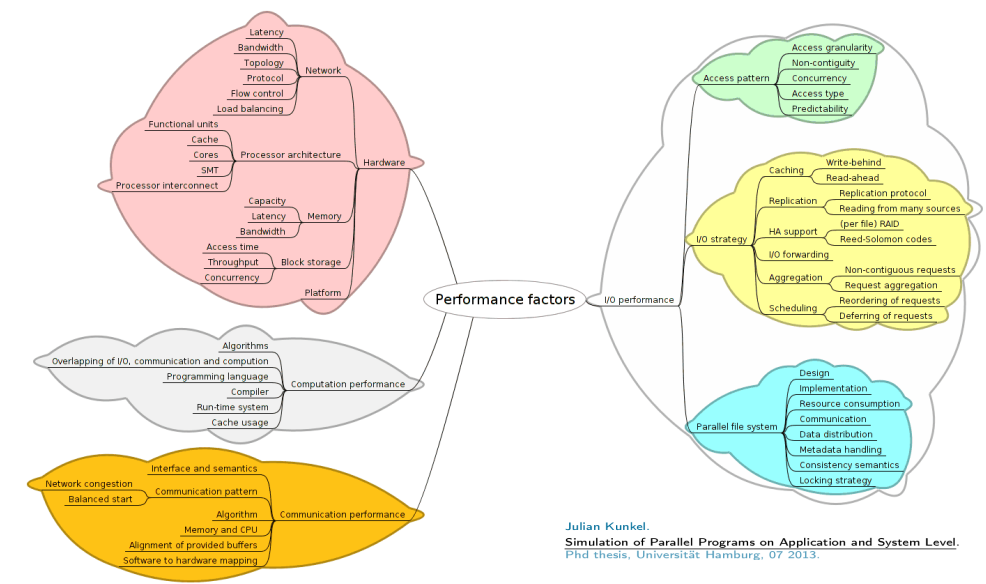
\includegraphics[scale=0.44]{fig/tree-perf}
\end{center}

\nocite{SOPPOAASLK13}

\end{frame}

\begin{frame}[fragile] {I/O Performance Factor -- Access Patterns}

\vspace*{0.6cm}

\begin{itemize}
\setlength\itemsep{1cm}

  \item The access pattern describes how\\ spatial access is performed over time.

  \item With an access pattern, the I/O of a single client process can be described, but also the actual observable patterns on the I/O servers, or on a single block device.

  \item The pattern on the I/O servers is caused by all clients and defines the performance of the I/O subsystems.

\end{itemize}

%\begin{textblock}{20}(40,20)
\begin{textblock}{2}(9,3)
   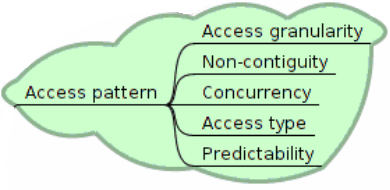
\includegraphics[scale=0.5]{fig/tree-io-ac-pat}
\end{textblock}

%\begin{picture}(50,50)
%\put(10,10){\hbox{\includegraphics[scale=0.3]{fig/tree-io-ac-pat}}}
%\put(200,-300){\hbox{\includegraphics[scale=0.3]{fig/tree-io-ac-pat}}}
%\end{picture}

%\begin{center}
%\includegraphics[scale=0.6]{fig/tree-io-ac-pat}
%\end{center}

\nocite{SOPPOAASLK13}

\end{frame}

\begin{frame}[fragile] {I/O Performance Factor -- I/O Strategy}

\begin{itemize}
\setlength\itemsep{0.5cm}

  \item In general, the mechanisms introduced here are orthogonal to the hardware and the architecture of the parallel file system.

  \item On the client-side, for instance, \\
  requests could already be tuned to improve \\
  the access pattern which will be observed \\
  on the servers.

  \item Similar to optimizations in communication, \\
  these strategies could be applied on any layer involved in I/O.

\end{itemize}

\begin{textblock}{0}(9,5)
   \includegraphics[scale=0.4]{fig/tree-io-strat}
\end{textblock}

%\begin{center}
%\includegraphics[scale=0.6]{fig/tree-io-strat}
%\end{center}

\nocite{SOPPOAASLK13}

\end{frame}

\begin{frame}[fragile] {I/O Performance Factor -- Parallel File System}

\begin{itemize}
\setlength\itemsep{0.5cm}

  \item Performance of a parallel file system highly depends on its design as it provides the frame for the deployed optimization strategies.

  \item Several aspects like consistency semantics also apply to higher level interfaces like domain specific I/O libraries.

\end{itemize}

%\begin{textblock}{0}(9,5)
%   \includegraphics[scale=0.5]{fig/tree-io-pfs}
%\end{textblock}

\begin{center}
\includegraphics[scale=0.5]{fig/tree-io-pfs}
\end{center}

\nocite{SOPPOAASLK13}

\end{frame}

\subsection{I/O Performance Factors}

\begin{frame}[fragile] {I/O Performance Tuning ``Rules of Thumb''}

\begin{itemize}
\setlength\itemsep{0.3cm}

  \item Use collectives when possible

  \item Use high-level libraries (e.g. HDF5 or PNetCDF) when possible

  \item A few large I/O operations are better than many small I/O operations

  \item Avoid unnecessary metadata operations, especially \texttt{stat()}

  \item Avoid writing to shared files with POSIX

  \item Avoid leaving gaps/holes in files to be written later

  \item Use tools like \textbf{Darshan} to check assumptions about behavior

\end{itemize}

%\begin{center}
%\includegraphics[scale=0.35]{fig/io-rules}
%\end{center}

\lr{tut145s3}

\end{frame}

\begin{frame}[fragile] {Assess and Optimize the Application I/O Performance}

\begin{itemize}
\setlength\itemsep{0.4cm}

    \item Develop general considerations about what influences the I/O performance

    \begin{itemize}
      \item What?
    \end{itemize}

    \item Analyze access pattern and define how it defines the performance of the I/O subsystems

    \begin{itemize}
      \item How?
    \end{itemize}

    \item Apply I/O strategies to improve the access pattern

    \begin{itemize}
      \item Which?
    \end{itemize}

    \item Identify options for the deployed optimization strategies in a specific parallel file system

    \begin{itemize}
      \item Which?
    \end{itemize}

\end{itemize}

\nocite{SOPPOAASLK13} \lr{skill-tree, Julian needs to address it.}

\end{frame}

\section{NetCDF}
\sectionIntro

\subsection{Introduction}

\begin{frame}[fragile] {NetCDF}

\begin{itemize}
\setlength\itemsep{0.4cm}

\item In a simple view, NetCDF is:

    \begin{itemize}
        \item A data mode.
        \item A file format.
        \item A set of APIs and libraries for various programming languages.
    \end{itemize}

\item Together, the data model, file format, and APIs support the creation, access, and sharing of scientific data.

\item NetCDF allows the user to describe multidimensional data and include metadata which further characterizes the data.

\item NetCDF APIs are available for most programming languages used in geosciences.

\end{itemize}

\nocite{netcdf}

\end{frame}

\subsection{Common Data form Language (CDL)}

\begin{frame}[fragile]{Common Data form Language (CDL)}

\begin{itemize}
\setlength\itemsep{0.3cm}

\item The notation used to describe a NetCDF object is called CDL (network Common Data form Language), which provides a convenient way of describing NetCDF datasets.

\begin{figure}
\centering
\begin{varwidth}{\linewidth}
\tiny{

\begin{verbatim}

netcdf short {
dimensions:
  latitude = 3 ;
  longitude = 2 ;
variables:
  float sfc_temp(latitude, longitude) ;
    sfc_temp:units = "celsius" ;
data:

 sfc_temp =
  10, 10.1,
  10.2, 10.3,
  10.4, 10.5 ;
}

\end{verbatim}
}
\end{varwidth}
%\caption{C++ code}
\end{figure}

\item The NetCDF system includes utilities for producing human-oriented CDL text files from binary NetCDF datasets and vice-versa.

\end{itemize}

\nocite{netcdf}

\end{frame}

\subsection{NetCDF Data Models}

\begin{frame}[fragile] {The Classic NetCDF Model}

\begin{itemize}

\item A NetCDF file (dataset) has a path name and possibly some dimensions, variables, global (file-level) attributes, and data values associated with the variables.

\end{itemize}

\begin{center}
\includegraphics[scale=0.6]{fig/netcdf-classic}
\end{center}

\nocite{netcdf}

\end{frame}

\begin{frame}[fragile] {NetCDF Data Models}

    \begin{itemize}

        \item Classic: Simplest model -- Dimensions, variables, attributes

        \item {\color{red}{Enhanced: More powerful model -- Adds groups, types, nesting}}

    \end{itemize}

    \begin{center}
    \includegraphics[scale=0.45]{fig/nc4-uml}
    \end{center}

\nocite{netcdf}

\end{frame}

\begin{frame}[fragile] {The NetCDF-4 Enhanced Data Model}

\begin{itemize}
\setlength\itemsep{0.4cm}

    \item The NetCDF-4 Enhanced Data Model, which is known as the ``Common Data Model'', is part of an effort of Unidata to find a common engineering language for the development of scientific data solutions.

    \item The model contains the variables, dimensions, and attributes of the classic data model, but adds:

    \begin{itemize}

        \item Groups -- A way of hierarchically organizing data, similar to directories in a Unix file system.\\[0.2cm]

        \item User-defined types -- The user can now define compound types (like C structures), enumeration types, variable length arrays, and opaque types.

    \end{itemize}

\end{itemize}

\nocite{netcdf}

\end{frame}

\begin{frame}[fragile] {The NetCDF-4 Enhanced Data Model}

    \begin{itemize}
    \setlength\itemsep{0.5cm}
        \item A file has a top-level unnamed group.
        \item Each group may contain one or more named subgroups, user-defined types, variables, dimensions, and attributes.
        \item Variables also have attributes.
        \item Variables may share dimensions, indicating a common grid.
        \item One or more dimensions may be of unlimited length.
    \end{itemize}

\nocite{netcdf}

\end{frame}

\subsection{Best Practices for Writing NetCDF Files}

\begin{frame}[fragile] {Experience-based ``Best Practices'' for Writing NetCDF Files}

    \begin{itemize}
    \setlength\itemsep{0.4cm}

        \item	Conventions
        \begin{itemize}
          \item Developers should be familiar with and use existing NetCDF conventions.
        \end{itemize}

        \item	Coordinate Systems
        \begin{itemize}
          \item Spatial and temporal location of data are supported by use of coordinate systems.
        \end{itemize}

        \item	Variable Grouping
        \begin{itemize}
          \item How you group data into variables can determine whether common analysis and visualization software can effectively use the data.
        \end{itemize}

        \item	Variable Attributes
        \begin{itemize}
          \item Conventional variable attributes supply necessary metadata.
        \end{itemize}

    \end{itemize}

\nocite{netcdf}

\end{frame}

\begin{frame}[fragile] {Experience-based ``Best Practices'' for Writing NetCDF Files}

    \begin{itemize}
    \setlength\itemsep{0.5cm}

        \item	Strings and Character Variables
        \begin{itemize}
          \item Use character data properly for representing text strings.
        \end{itemize}

        \item Calendar Date and Time
        \begin{itemize}
          \item Represent calendar dates and times with standards and conventions.
        \end{itemize}

        \item	Packed Data Values
        \begin{itemize}
          \item Conventions for packing numeric data to save space have some subtleties.
        \end{itemize}

        \item Missing Data Values
        \begin{itemize}
          \item To indicate that data values are missing, invalid, or not written, special values are conventionally used.
        \end{itemize}

    \end{itemize}

\nocite{netcdf}

\end{frame}

\subsection{Climate and Forecast (CF) Conventions}

\begin{frame}[fragile] {Climate and Forecast (CF) Conventions}

\begin{itemize}
\setlength\itemsep{0.3cm}

\item The Climate and Forecast (CF) conventions are metadata conventions for earth science data, intended to promote the processing and sharing of files created with the NetCDF API.

% \item The CF conventions define metadata that are included in the same file as the data (thus making the file ``self-describing'').

\item The purpose of the CF conventions is to require conforming datasets to contain sufficient metadata that they are self-describing:

    \begin{itemize}

      \item Each variable in the file has an associated description of what it represents, including physical units if appropriate.

      \item Each value can be located in space (relative to earth-based coordinates) and time.

    \end{itemize}

\item The CF conventions enable users of data from different sources to decide which data are comparable and allows building applications with powerful extraction, regridding, and display capabilities.

\end{itemize}

\end{frame}

\section{Parallel I/O in NetCDF-4}
\sectionIntro

\begin{frame}[fragile] {Parallel I/O}

\begin{itemize}
\setlength\itemsep{0.1cm}

  \item Parallel I/O allows each processor in a multi-processor system to read and write data from multiple processes to a common file independently.

  \begin{center}
  \includegraphics[scale=0.5]{fig/pnetcdf}
  \end{center}

  \item Data-intensive scientific applications use parallel I/O software to access files.

  \item In HPC, increasing demands in the I/O system can cause bottlenecks. Parallel I/O plays a fundamental role to balance the fast increase in computational power and the progress of processor architectures.

  \item Used properly, parallel I/O allows users to overcome I/O bottlenecks in HPC environments.

\end{itemize}

\end{frame}

\begin{frame}[fragile]{Parallel I/O in NetCDF-4}

\begin{itemize}
\setlength\itemsep{0.6cm}

  \item NetCDF-4 provides parallel file access to both classic and NetCDF-4/HDF5 files.

  \item The parallel I/O to NetCDF-4 files is achieved through the HDF5 library while the parallel I/O to classic files is through PNetCDF.

  \item NetCDF-4 exposes the parallel I/O features of HDF5.
    \begin{itemize}
    \item HDF5 provides easy-to-use parallel I/O feature.
    \end{itemize}

  \item Parallel NetCDF uses MPI I/O to perform parallel I/O. It is a complete rewrite of the core C library using MPI I/O instead of POSIX.

\end{itemize}

\end{frame}

\begin{frame}[fragile]{Using Parallel I/O in NetCDF-4}

\begin{itemize}
\setlength\itemsep{0.4cm}

  \item Special \verb|nc_create_par| and \verb|nc_open_par| functions are used to create/open a NetCDF file.

  \item The files they open are normal NetCDF-4/HDF5 files, but these functions also take MPI parameters.

  \item The parallel access associated with these functions is not a characteristic of the data file, but the way it was opened. The data file is the same, but using the parallel \verb|open/create| function allows parallel I/O to take place.

\end{itemize}

\begin{figure}
\centering
\begin{varwidth}{\linewidth}
{ \tiny

\begin{verbatim}

EXTERNL int
nc_create_par(const char *path, int cmode, MPI_Comm comm,
               MPI_Info info, int *ncidp);

EXTERNL int
nc_open_par(const char *path, int mode, MPI_Comm comm,
             MPI_Info info, int *ncidp);

\end{verbatim}

}
\end{varwidth}
\end{figure}

\end{frame}

\begin{frame}[fragile]{Collective and Independent Operations with Parallel I/O}

\begin{itemize}
\setlength\itemsep{0.4cm}

  \item In MPI programs, I/O may be collective or independent.

    \begin{itemize}
      \item Collective: It must be done by all processes at the same time
      \item Independent: It can be done by any process at any time.
    \end{itemize}

  \item All NetCDF metadata writing operations are collective. That is, all creation of groups, types, variables, dimensions, or attributes.

  \item Data reads and writes (ex. calls to \verb|nc_put_vara_int| and \verb|nc_get_vara_int|) may be independent (the default) or collective. To make writes to a variable collective, call the \verb|nc_var_par_access| function.

\end{itemize}

\begin{figure}
\centering
\begin{varwidth}{\linewidth}
{ \tiny

\begin{verbatim}

/* Use these with nc_var_par_access(). */
#define NC_INDEPENDENT 0
#define NC_COLLECTIVE 1

EXTERNL int
nc_var_par_access(int ncid, int varid, int par_access);

\end{verbatim}

}
\end{varwidth}
\end{figure}

\end{frame}

\begin{frame}[fragile]{Collective and Independent Operations with Parallel I/O}

\begin{itemize}

  \item You must build NetCDF-4 properly to take advantage of parallel features.

  \begin{itemize}
  \setlength\itemsep{0.3cm}

    \item HDF5 must be built with \verb|--enable-parallel|.

    \item Typically the CC environment variable is set to mpicc, and the FC to mpifc (or some local variant.) You must build HDF5 and NetCDF-4 with the same compiler and compiler options.

    \item The NetCDF configure script will detect the parallel capability of HDF5 and build the NetCDF-4 parallel I/O features automatically. No configure options to the netcdf configure are required.

    \item For parallel builds you must include \verb|"netcdf_par.h"| before (or instead of) \verb|netcdf.h|.

    \item Parallel tests are run by shell scripts. For testing to work on your platform the \verb|mpiexec| utility must be supported.

    \item Parallel I/O is tested in \verb|nc_test4/tst_parallel.c|, \verb|nc_test4/tst_parallel2.c|, and \verb|nc_test4/tst_parallel3.c|, and other programs, if the \verb|--enable-parallel-tests| option to configure is used.

  \end{itemize}

\end{itemize}

\end{frame}

\begin{frame}[fragile] {Parallel I/O Example -- Part I}

\begin{figure}
\centering
\begin{varwidth}{\linewidth}
{ \tiny

\begin{verbatim}

/* Initialize MPI. */
    MPI_Init(&argc,&argv);
    MPI_Comm_size(MPI_COMM_WORLD, &mpi_size);
    MPI_Comm_rank(MPI_COMM_WORLD, &mpi_rank);
    MPI_Get_processor_name(mpi_name, &mpi_namelen);

    if (mpi_rank == 1)
       printf("\n*** tst_parallel testing very basic parallel access.\n");

    /* Create a parallel netcdf-4 file. */
    if ((res = nc_create_par(FILE, NC_NETCDF4|NC_MPIIO, comm,
			     info, &ncid))) ERR;

    /* Create two dimensions. */
    if ((res = nc_def_dim(ncid, "d1", DIMSIZE, dimids))) ERR;
    if ((res = nc_def_dim(ncid, "d2", DIMSIZE, &dimids[1]))) ERR;

    /* Create one var. */
    if ((res = nc_def_var(ncid, "v1", NC_INT, NDIMS, dimids, &v1id))) ERR;

    if ((res = nc_enddef(ncid))) ERR;

\end{verbatim}

}
\end{varwidth}
\end{figure}

\end{frame}

\begin{frame}[fragile] {Parallel I/O Example -- Part II}

\begin{figure}
\centering
\begin{varwidth}{\linewidth}
{ \tiny

\begin{verbatim}

    /* Set up slab for this process. */
    start[0] = mpi_rank * DIMSIZE/mpi_size;
    start[1] = 0;
    count[0] = DIMSIZE/mpi_size;
    count[1] = DIMSIZE;

    /* Create phoney data. We're going to write a 24x24 array of ints,
       in 4 sets of 144. */
    for (i=mpi_rank*QTR_DATA; i < (mpi_rank+1)*QTR_DATA; i++)
       data[i] = mpi_rank;

    /*if ((res = nc_var_par_access(ncid, v1id, NC_COLLECTIVE)))
      ERR;*/
    if ((res = nc_var_par_access(ncid, v1id, NC_INDEPENDENT))) ERR;

    /* Write slabs of phoney data. */
    if ((res = nc_put_vara_int(ncid, v1id, start, count,
			       &data[mpi_rank*QTR_DATA]))) ERR;

    /* Close the netcdf file. */
    if ((res = nc_close(ncid)))	ERR;

    /* Shut down MPI. */
    MPI_Finalize();

    return 0;

\end{verbatim}

}
\end{varwidth}
\end{figure}

\end{frame}

\section{Research Activities}
\sectionIntro

\subsection{}

\begin{frame}[fragile] {Describe ongoing research activities in high-performance storage}

\begin{itemize}

  \item
    \begin{itemize}
        \item TODO
        \item
    \end{itemize}
  \item
    \begin{itemize}
      \item
    \end{itemize}
\end{itemize}

\end{frame}

\begin{frame}[fragile] {Previous Learning Objectives}

\begin{itemize}

    \item Describe the general layers involved in I/O on a supercomputer
    \item Analyse the implications of parallel I/O on application efficiency
    \item Identify typical I/O performance issues and their causes
    \item Design a data model for NetCDF/CF
    \item Read, analyse, and write NetCDF files in a metadata-aware manner
    \item Visualise and regrid field constructs within NetCDF

\end{itemize}

\end{frame}

\begin{frame}[allowframebreaks]{Bibliography}

{

\tiny

\bibliographystyle{alpha}
\bibliography{io}

}

\end{frame}

\acknowledgement

\end{document}
